\subsection*{Solution Design}
The second prototype will focus on improving the method of sending the chunked data. This is necessary improvement, as in the event of many packets being dropped during a transfer; it will not be until the end of the transfer until the lost packets can be recovered.

To solve this without sending and waiting for acknowledgments for each packet (re-implementing TCP) a different method must be implemented. On smaller transfers the number of lost packets to recover from will be less than a larger transfer, grouping several chunks into a block of chunks then verifying each block will likely solve this issue. A sequence diagram example of a complete transfer is shown in Figure~\ref{fig:p2-sequence}.

\newpage
\begin{figure}[h!]
    \centering
    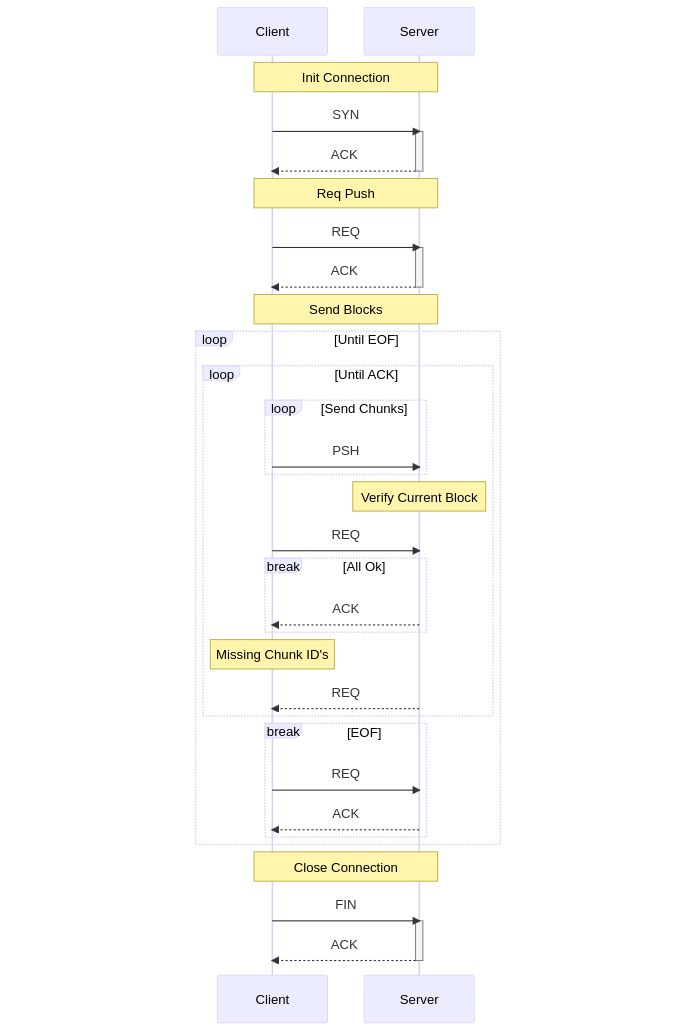
\includegraphics[width=0.9\linewidth]{p2-sequence.png}
    \caption{Prototype Two Sequence Diagram}
    \label{fig:p2-sequence}
\end{figure}
\newpage

In prototype one during the end of a transfer only three request types were sent: request to send a file, the file data and a verify packet to check if any chunks were needed to be resent. In this prototype a new request type has been added for marking the end-of-file (EOF) and ending the file transfer. The request for verification will not end the transfer; instead it is repurposed for checking for missing chunks for the current group. This will reduce the complexity of needing the server to keep a record of the blocks.

The existing protocol packet fields from prototype (headers and metadata) will stay the same. Both the client and server code will need to be altered to handle the new request type and at the client side keeping track of how many chunks are sent per block will need to be implemented. Figure~\ref{lst:p2d-offset-variables} shows the variables required for calculating blocks

\begin{lstlisting}[caption={Prototype Two Offset Variables},label=lst:p2d-offset-variables,breaklines,numbers=left,language=go]
var lastChunkID uint64 = 0
var seekOffset int = 0

chunkIDToOffset := make(map[uint64]int)

eof := false
missingChunks := make([]uint64, 0)
\end{lstlisting}


\subsection*{Testing}
After running the first test; an issue in the code discovered and had to be fixed. This is listed below (with git commit hashes):

\begin{itemize}
    \item (cae32ef) file reader cursor position not set back after a requested resend, causing incorrect data to be sent on next PSH. Fixed by seeking to stored seek offset before reading
\end{itemize}

In the first test sending a single file resulted in a higher overhead than the previous prototype, it also now has a higher overhead compared to all the tested existing solutions now showing "6.24\%". This means that implementing the transfer in blocks increased the overhead due to more packets being sent, which is shown in the results Table~\ref{tab:prototypes-test-results} going from "39" packets to "45".

In the text and photos tests prototype two still performed better than FTP and SMB2, however worse than rsync and the first prototype having "2.44\%" more overhead when transferring text and "0.19\%" more when transferring photos. This shows that the extra overhead created for handling validation of each block creates more impact on smaller files. Looking at the synthetic 1KB files test, shows the overhead to be "6.54\%" greater than prototype one. This indicates the same issue found in the text and photos test results.

In this prototype, test transfer speeds have reduced from prototype one, for example in the photos test it went from "1.9Gbps" down to "255.9Mbps", whilst slower than rsync's 1.0Gbps it reached a much greater speed than both FTP and SMB2. It likely that the extra validation added can be optimised at the software side in the last prototype.

Adding the extra message to mark a file as EOF (end-of-file), has been proved to create more overhead when sending many files. However this extra feature should allow for longer transfers to handle missing data sooner; rather than waiting until the end. The next prototype will need to ensure packet size is kept to a minimum, to reduce this overhead.

During testing an issue was discovered during transfers with multiple blocks, when they arrive out-of-order. This issue causes the chunks for different blocks to be captured incorrectly causing a corrupted file. To handle this prototype three will need to allow the receiver of a transfer to see which current chunk relates to what block. This will however increase the size of each chunk packet, but is a necessary increase in overhead for vital error checking.

Allowing the server to also know the maximum number of chunks per block could also allow memory to be pre-allocated allowing for less time to be taken allocating memory and potentially reducing the number of dropped packets during a transfer on a lower spec machine.

Due to the seen higher overhead created in both prototype one and two, the field sizes need to be reduced. Reserving 8 bytes each for the header, metadata and payload lengths causes quite a large amount of reserved space. These could be reduced from uint64 fields to uint32 reducing each field from taking 8 bytes to only 4 bytes. Also removing the metadata field as discussed in prototype one's testing would remove the need for one of the length fields.
